% Fig 9: Extraction ratio and min-entropy vs number of frames
\begin{figure}[t]
\centering
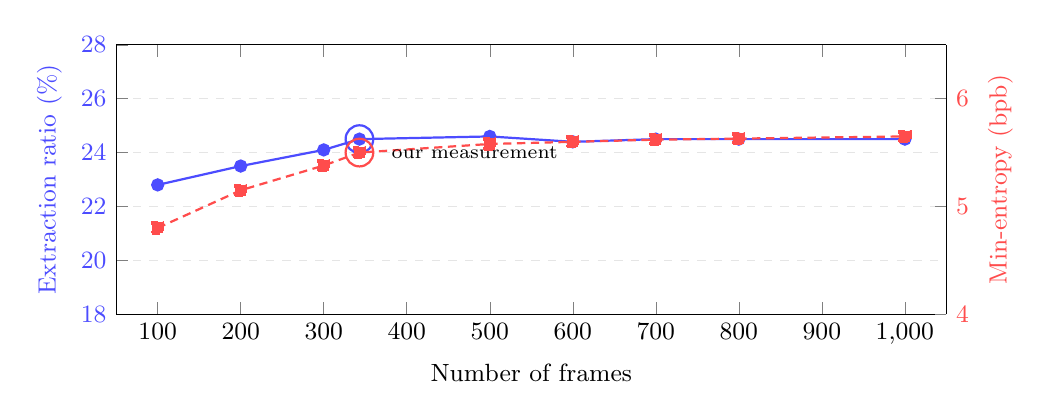
\begin{tikzpicture}
\begin{axis}[
  width=\columnwidth,
  height=5cm,
  xlabel={Number of frames},
  xlabel style={font=\small},
  axis y line*=left,
  ylabel={Extraction ratio (\%)},
  ylabel style={font=\small, blue!70},
  yticklabel style={font=\small, blue!70},
  xticklabel style={font=\small},
  xmin=50, xmax=1050,
  ymin=18, ymax=28,
  ymajorgrids=true,
  grid style={dashed, gray!20},
]
\addplot[thick, blue!70, mark=*, mark size=2pt] coordinates {
  (100, 22.8) (200, 23.5) (300, 24.1) (343, 24.5) (500, 24.6)
  (600, 24.4) (700, 24.5) (800, 24.5) (1000, 24.5)
};
\label{pgf:ratio}
% Mark our measurement point
\draw[blue!70, thick] (axis cs:343, 24.5) circle (5pt);
\end{axis}

\begin{axis}[
  width=\columnwidth,
  height=5cm,
  axis y line*=right,
  axis x line=none,
  ylabel={Min-entropy (bpb)},
  ylabel style={font=\small, red!70},
  yticklabel style={font=\small, red!70},
  xmin=50, xmax=1050,
  ymin=4, ymax=6.5,
]
\addplot[thick, red!70, mark=square*, mark size=2pt, densely dashed] coordinates {
  (100, 4.80) (200, 5.15) (300, 5.38) (343, 5.50) (500, 5.58)
  (600, 5.60) (700, 5.62) (800, 5.63) (1000, 5.65)
};
\label{pgf:entropy}
% Mark our measurement point
\draw[red!70, thick] (axis cs:343, 5.50) circle (5pt);
\node[font=\scriptsize, anchor=west] at (axis cs:370, 5.50) {our measurement};
\end{axis}
\end{tikzpicture}

\vspace{2pt}
{\scriptsize \ref{pgf:ratio}~Extraction ratio \quad \ref{pgf:entropy}~Min-entropy (projected)}

\caption{Extraction quality vs.\ number of input frames. Both extraction ratio (solid, left axis) and min-entropy (dashed, right axis) converge with increasing sample size. Our measurement (343~frames, circled) yields 24.5\% and 5.50~bpb. Extrapolation to 1{,}000 frames suggests marginal improvement to $\approx$5.65~bpb, still below quantum and OS sources.}
\label{fig:extraction-sensitivity}
\end{figure}
